\chapter{Study and realization of the Sprint 2}
\minitoc
\newpage


\setcounter{secnumdepth}{2} % Resume counting the sections for the toc with a depth of 2 (Sections and sub-sections)
% ----------------------------------- SECTIONS (v) ----------------------------------- %
% ----------------------- Deployment process ----------------------- %
\section{Backlog of the sprint}
This sprint is focused on the implementation of specific features in the application that directly involve the end user (the HR Manager). These features (such as dropdown selection of job and field, skill filtering and selection, task fetching, job description generation, etc.) leverage the data infrastructure set up in Sprint 1.

$ \rightarrow $ In other words, Sprint 1 is about setting up the data backend, while Sprint 2 is about creating the user-facing features that interact with that data.
However, it's worth noting that in real-world development, there can be some overlap and iteration between these stages. For example, while implementing the features in Sprint 2, you might discover the need for additional data structuring or modifications in the database, leading to some revisiting of the work done in Sprint 1. This is a common part of the iterative nature of agile development methodologies like Scrum.

\renewcommand{\arraystretch}{1.5}
\setlength{\tabcolsep}{10pt}


\begin{xltabular}{1.2\textwidth}{
    | >{\hsize=0.8\hsize\raggedright\arraybackslash}X
    | >{\hsize=0.8\hsize\raggedright\arraybackslash}X
    | >{\hsize=1.8\hsize\raggedright\arraybackslash}X
    | >{\hsize=0.6\hsize\raggedright\arraybackslash}X |}
\caption{Sprint 2 Backlog} \\
\hline
\rowcolor{primary} \textbf{User Story} & \textbf{Subtask} & \textbf{Description} & \textbf{Estimated Time} \\
\hline
\endfirsthead
\multicolumn{4}{c}%
{\tablename\ \thetable\ -- \textit{Continued from previous page}} \\
\hline
\rowcolor{primary} \textbf{User Story} & \textbf{Subtask} & \textbf{Description} & \textbf{Estimated Time} \\
\hline
\endhead
\hline \multicolumn{4}{r}{\textit{Continued on next page}} \\
\endfoot
\hline
\endlastfoot
% Your table content here
As an HR Manager, I want to select a job category and the associated specialized field so that I can define roles and responsibilities. & Design and implement a dynamic dropdown feature for job category selection & Implement a feature that allows HR Managers to select an origin, a personnel category, a personnel type, a job category, and if available, a specialized field, each from a dropdown menu. Each selection influences the options available in the next dropdown. & 2 days \\
\hline
 & Connect the dropdown selections to the Airtable database & Establish a connection between the dropdown selection feature and the Airtable database to fetch the relevant data. This involves pulling the data for each dropdown based on the user's previous selections. & 2 days \\
\hline
As an HR Manager, I want to filter and select the necessary skills for the chosen job category so that I can ensure the necessary competencies for the job are outlined. & Design and implement a web service that fetches related skills & Develop a feature that fetches skills related to the selected job category (and specialized field if selected) from the Airtable database. & 2 days \\
\hline
 & Integrate Algolia search engine for skill filtering and searching & Incorporate Algolia search engine capabilities to enable HR Managers to filter and search through the skills. & 3 days \\
\hline
As an HR Manager, I want to fetch and select the tasks related to the chosen skills so that I can ensure all necessary tasks for the job are included. & Design and implement a web service that fetches related tasks & Develop a feature that fetches tasks related to the selected skills from the Airtable database. & 5 days \\
\hline
 & Integrate Algolia search engine for task filtering and searching & Incorporate Algolia search engine capabilities to enable HR Managers to filter and search through the tasks. & 2 days \\
\hline
As an HR Manager, I want to generate the job description using the selected skills and tasks so that I can have a comprehensive job description. &Implement a feature that generates a job description using the GPT-3 API & Develop a feature that generates a job description using the GPT-3 API based on the selected skills and tasks. & 5 days \\
\hline
 & Display the generated job description for the HR Manager & Develop a feature that displays the generated job description for the HR Manager. & 1 day \\
\hline
 & Implement a feature for updating/deleting the job description & Develop features that allow HR Managers to delete or update the generated job description. & 1 day \\
\hline
\end{xltabular}


\newpage
\section{Functional Specification}
In this sub-section, we present the analysis phase that answers the question “what does the system do”. The answer to this question is translated by the presentation of the diagram of the use cases and the textual description of each of them.

\subsection{Use Case Diagram}
The use case would typically include the following main actors and their interactions with the system :


\begin{figure}[H]
    \centering
    \makebox[\textwidth]{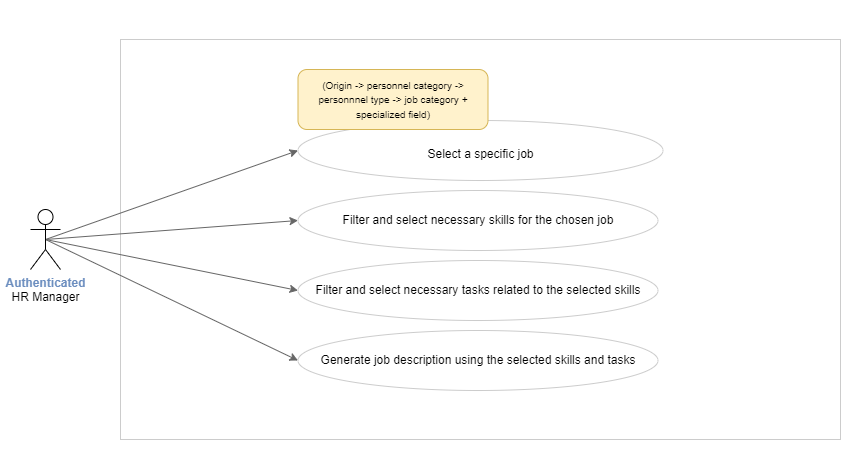
\includegraphics[width=\linewidth]{src/assets/images/HRMUseCase2.drawio.png}}
    \caption{ Use Case Diagram For Sprint 2 }
    \label{fig:Sprint2_UseCaseDiagram}
\end{figure}

\subsection{Textual Description of the Use Cases}
\subsubsection{\underline{Use Case 1: Select Job Category and Specialized Field}}
In this use case, the HR Manager interacts with the system to select a job category and, if applicable, a specialized field. The system provides drop-down lists for the HR Manager to select the desired options. The system fetches and displays the relevant personnel categories, personnel types, and job categories based on the HR Manager's selections. If the chosen job category has associated specialized fields, the system presents these options in an additional drop-down list.


\begin{table}[H]
    \renewcommand{\arraystretch}{1.5}%
    \caption{Use Case 1: Select Job Category and Specialized Field}
    \centering
    \medskip
    \small
    \begin{tabularx}{1.2\textwidth} {
            | >{\hsize=0.4\hsize\raggedright\arraybackslash}X
            | >{\hsize=1.6\hsize\raggedright\arraybackslash}X |}
        \hline
        \textbf{Title} & Select Job Category and Specialized Field \\
        \hline
        \textbf{Main Actor} & HR Manager \\
        \hline
        \textbf{Summary} & HR Manager selects a Job Category, and potentially a Specialized Field, for the new Job Description from dynamic dropdowns \\
        \hline
        \textbf{Preconditions} & HR Manager is authenticated and on the job description creation page \\
        \hline
        \textbf{Main Success Scenario} & 1. HR Manager selects the origin from the first dropdown. \\
        & 2. System fetches all the personnel categories of that origin and displays them in the second dropdown. \\
        & 3. HR Manager selects the personnel category of interest. \\
        & 4. System fetches all the personnel types related to that personnel category and displays them in the third dropdown. \\
        & 5. HR Manager selects the personnel type of interest. \\
        & 6. System fetches all job categories related to that personnel type and displays them in the fourth dropdown. \\
        & 7. HR Manager selects the job category of interest. \\
        & 8. If there are specialized fields related to the chosen job category, system fetches them and displays them in the fifth dropdown. \\
        & 9. HR Manager selects the specialized field of interest, if applicable. \\
        \hline
        \textbf{Postconditions} & The Job Category and Specialized Field (if applicable) have been selected for the new Job Description. The system is ready to move to the next step of the job description creation process (filtering and selecting skills). \\
        \hline
        \textbf{Alternative Scenarios} & 1. If no specialized fields exist for a job category, the HR Manager can proceed to the next step directly after selection.\\
        & 2. The HR Manager can change the origin, personnel category, personnel type, or job category anytime, with the system updating the dropdowns dynamically. \\
        & 3. The HR Manager can cancel the process anytime, with changes not being saved for future sessions. \\
        \hline
    \end{tabularx}
    \normalsize
\end{table}

\subsubsection{\underline{Use Case 2: Filter and Select Skills for Chosen Job Category }}
After the HR Manager has selected a job category (and a specialized field, if applicable), they proceed to select the necessary skills for the job. The system fetches the skills related to the selected job category from the database and displays them for the HR Manager. They can filter and search through the skills using Algolia's search engine capabilities embedded in the system.

\vspace{1cm}

\begin{xltabular}{1.2\textwidth}{|>{\hsize=0.4\hsize}X|>{\hsize=1.6\hsize}X|}
    \caption{Use Case 2: Filter and Select Skills for Chosen Job Category} \\
    \hline
    \textbf{Title} & Filter and Select Skills for Chosen Job Category \\
    \hline
    \textbf{Main Actor} & HR Manager \\
    \hline
    \textbf{Summary} & The HR Manager filters and selects relevant skills from a list retrieved by the system based on the chosen job category and potentially specialized field. \\
    \hline
    \textbf{Preconditions} & HR Manager is authenticated and is on the job description creation page. A job category (and potentially specialized field) has been selected. \\
    \hline
    \textbf{Main Success Scenario} & 1. The system retrieves and displays a list of skills relevant to the chosen job category and potentially specialized field. The skills are presented in a searchable format. \\
    & 2. HR Manager uses the search functionality provided by Algolia to find the required skills, the system displays the corresponding results dynamically. \\
    & 3. HR Manager selects the skills relevant to the job description from the results displayed. Each selected skill is added to a list of chosen skills. \\
    & 4. HR Manager can remove any selected skill from the list if they decide it is not appropriate. \\
    & 5. After selecting all required skills, HR Manager clicks on the 'Confirm Skills' button. \\
    & 6. The system stores the selected skills associated with the job description and proceeds to the next step of the job description creation process. \\
    \hline
    \textbf{Postconditions} & The selected skills for the job description have been saved by the system. HR Manager is ready to proceed to the next step of selecting tasks related to the chosen skills. \\
    \hline
    \textbf{Alternative Scenarios} & 1. If a specific skill isn't found via search, the HR Manager can manually scroll through the list to select it. \\
    & 2. If the HR Manager changes the job category or specialized field, the system resets the selected skills and updates the list accordingly. \\
    & 3. The HR Manager can cancel the process at any time, with the current selections not being saved for future sessions. \\
    \hline
\end{xltabular}

\subsubsection{\underline{Use Case 3: Fetch and Select Tasks for Chosen Skills }}
In this use case, the HR Manager selects the tasks related to the chosen skills. The system fetches and displays the tasks associated with the selected skills from the database. The HR Manager can search and filter through these tasks using Algolia's search engine capabilities.



\begin{xltabular}{1.2\textwidth}{|>{\hsize=0.4\hsize}X|>{\hsize=1.6\hsize}X|}
    \caption{Use Case 3: Fetch and Select Tasks for Chosen Skills} \\
    \hline
    \textbf{Title} & Fetch and Select Tasks for Chosen Skills \\
    \hline
    \textbf{Main Actor} & HR Manager \\
    \hline
    \textbf{Summary} & After selecting skills for the chosen job category, the HR Manager is presented with the associated tasks automatically fetched by the system. The HR Manager then reviews and selects the tasks that suit the job description they're creating \\
    \hline
    \textbf{Preconditions} & \begin{itemize} \item The HR Manager has successfully logged into the system. \item The HR Manager has selected a job category and specialized field. \item The HR Manager has selected skills for the chosen job category. \end{itemize} \\
    \hline
    \textbf{Main Success Scenario} & 1. The system retrieves and displays a list of tasks relevant to the chosen skills, with each task represented as a card. The tasks are presented in a searchable format powered by Algolia. \\
    & 2. The HR Manager uses the search functionality to find the required tasks. The system dynamically updates and displays the corresponding results. \\
    & 3. The HR Manager selects the tasks relevant to the job description from the results displayed. Each selected task is added to a list of chosen tasks. \\
    & 4. The HR Manager can remove any selected task from the list if they decide it is not appropriate. \\
    & 5. After selecting all required tasks, the HR Manager clicks on the 'Next' button in the page view. \\
    & 6. The system stores the selected tasks associated with the job description and proceeds to the next step of the job description creation process. \\
    \hline
    \textbf{Postconditions} & \begin{itemize} \item Tasks associated with the chosen skills are successfully fetched. \item HR Manager has selected the tasks that are suitable for the job description. \end{itemize} \\
    \hline
    \textbf{Alternative Scenarios} & 1. The HR Manager reviews the list of tasks but doesn't select any. \\
    & 2. The HR Manager clicks the "Confirm Task Selection" button. \\
    & 3. The system prompts a message to select at least one task. \\
    \hline
\end{xltabular}

\subsubsection{\underline{Use Case 4: Generate Job Description}}
Finally, the HR Manager generates the job description using the selected skills and tasks. The system uses the GPT-3 API to generate a comprehensive job description based on the selected skills and tasks. The HR Manager can view the generated job description, and if necessary, delete or update it.

\newpage
\begin{xltabular}{1.2\textwidth}{|>{\hsize=0.5\hsize}X|>{\hsize=1.5\hsize}X|}
    \caption{Use Case 4: Generate Job Description} \\
    \hline
    \textbf{Title} & Generate Job Description \\
    \hline
    \textbf{Main Actor} & HR Manager \\
    \hline
    \textbf{Summary} & The HR Manager generates the job description based on the chosen job category, skills, and tasks \\
    \hline
    \textbf{Preconditions} & The HR Manager has successfully selected a job category, specified skills, and chosen tasks. \\
    \hline
    \textbf{Main Success Scenario} & 1. The HR Manager clicks the 'Generate Job Description' button. \\
    & 2. The system calls the GPT API and generates a detailed job description based on the selected information. \\
    & 3. The system displays the generated job description to the HR Manager. \\
    & 4. The HR Manager can download, print, modify, regenerate, or delete the job description. \\
    & 5. Any modification or new generation of job description is saved in the Firestore database. \\
    & 6. The HR Manager can return to the page where job descriptions are displayed and consult, modify or delete any of them. \\
    \hline
    \textbf{Postconditions} & The job description is generated, saved in the database, and available for the HR Manager's use. \\
    \hline
    \textbf{Alternative Scenarios} & If the HR Manager opts not to generate a job description, the system retains the provided information, allowing the HR Manager to resume from the same point later. \\
    \hline
\end{xltabular}


\section{Design} 
In this sub-section, we will present the different detailed Activity Diagrams + Sequence diagrams for the first sprint.

\newpage
\subsection{Detailed Activity Diagrams}
\subsubsection{Use Case 1: Select Job Category and Specialized Field} 


\begin{figure}[H]
    \centering
    \makebox[\textwidth]{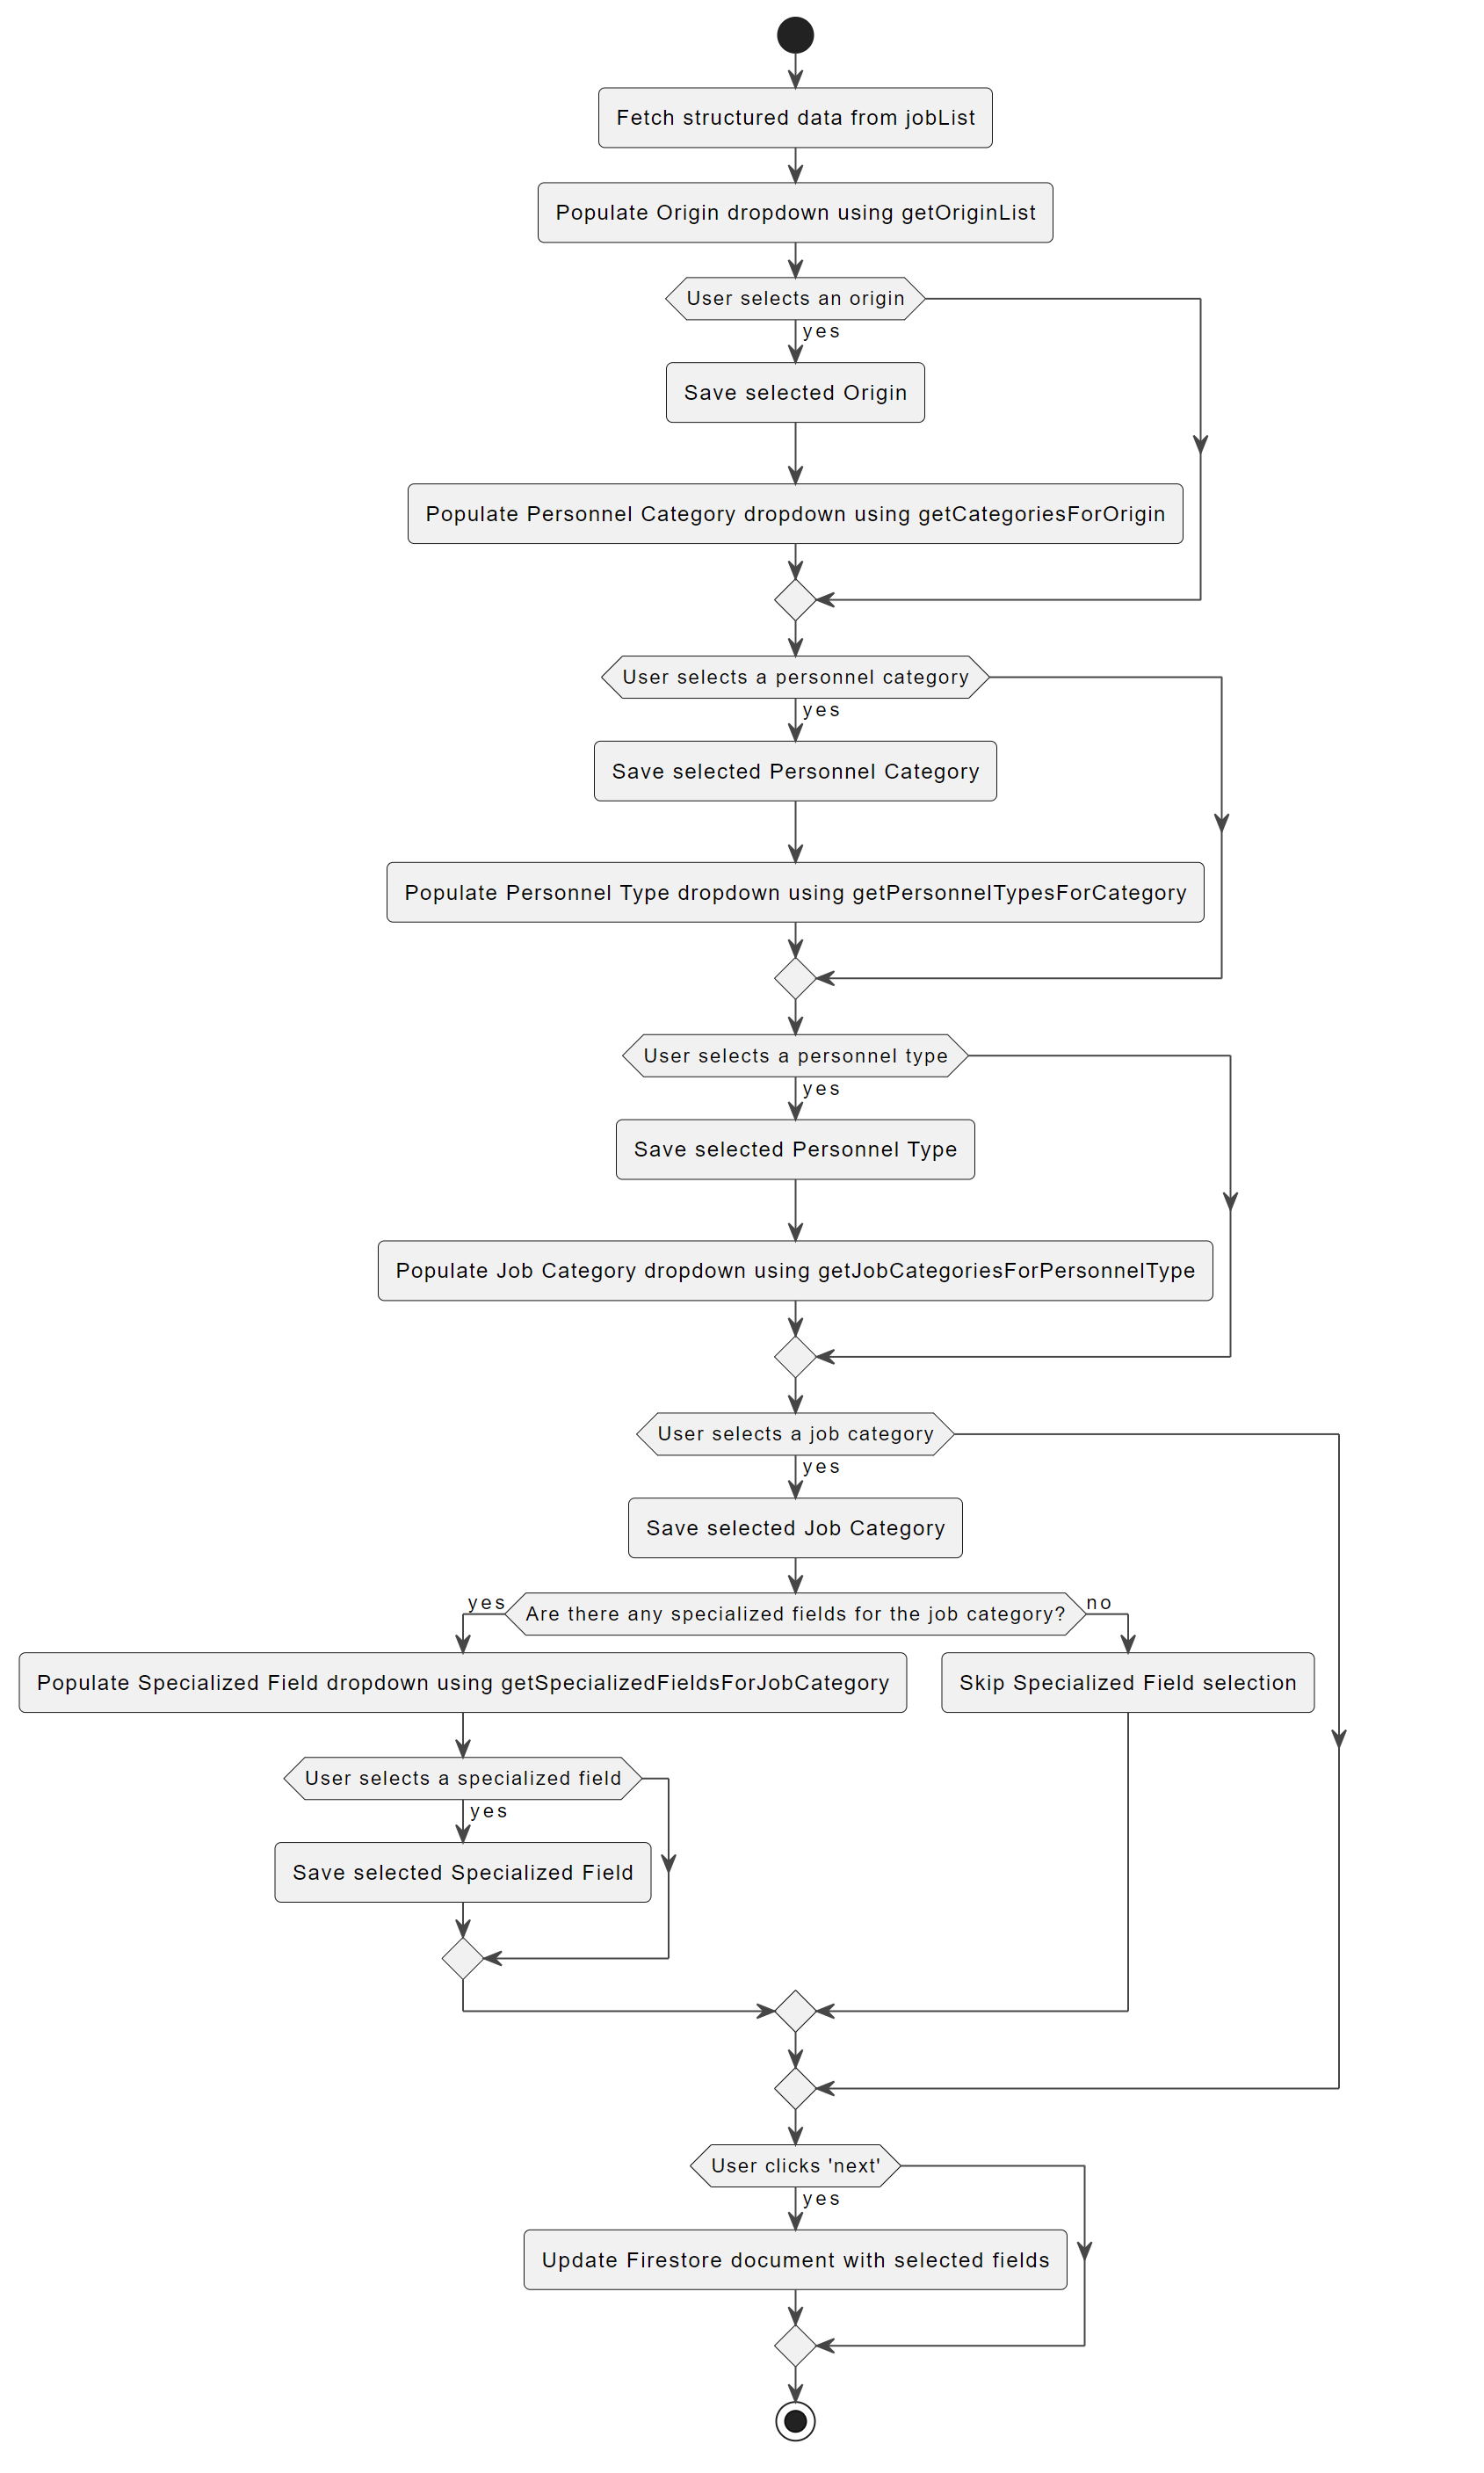
\includegraphics[width=0.8\linewidth]{src/assets/images/sprint2UseCase1.png}}
    \caption{ Activity Diagram for the Select Job Category and Specialized Field Use-Case }
    \label{fig:UseCase1Sprint2_Activity_Diagram}
\end{figure}



\subsection*{Description}
The first use case activity diagram outlines the complex, but user-friendly process of the job category and related field selection. It begins with an essential step of pulling structured job data from a Firestore database, making the app aware of the available options that can be presented to the HR manager.

Once this data is successfully fetched, the system populates the first dropdown menu which is the Origin field. The HR Manager selects an option from the Origin dropdown, which triggers an event in the system that saves this selection as a variable. This variable is important because it determines the contents of the subsequent dropdowns.

The selection from the Origin field is then used by the system to populate the next dropdown, which is the Personnel Category. The options in the Personnel Category dropdown are dependent on the Origin chosen. After the HR Manager makes a selection, this too is saved as a variable within the system.

Continuing this cascading pattern, the Personnel Type dropdown is populated next, with options that correspond to the selected Personnel Category. The HR Manager makes a selection from these options and the choice is again saved by the system.

The Job Category dropdown is the next to be populated, its options are entirely dependent on the Personnel Type selected. The HR Manager's choice from this dropdown is also stored in the system.

If the chosen Job Category has any Specialized Fields associated with it, another dropdown is shown, populated with these specialized fields. The HR Manager can then select from these options and the selected specialized field is saved. If there are no specialized fields related to the chosen Job Category, the system intelligently skips this step to streamline the user's experience.

Once all the appropriate selections have been made, the HR Manager can click on the 'Next' button. The act of clicking this button triggers a system event that updates the Firestore document with the selected fields. This ensures that the HR Manager's choices are saved and can be used in the future, maintaining the state of the application for the user.

\subsubsection{Use Case 2: Filter and Select Skills for Chosen Job Category} 
\begin{figure}[H]
    \centering
    \makebox[\textwidth]{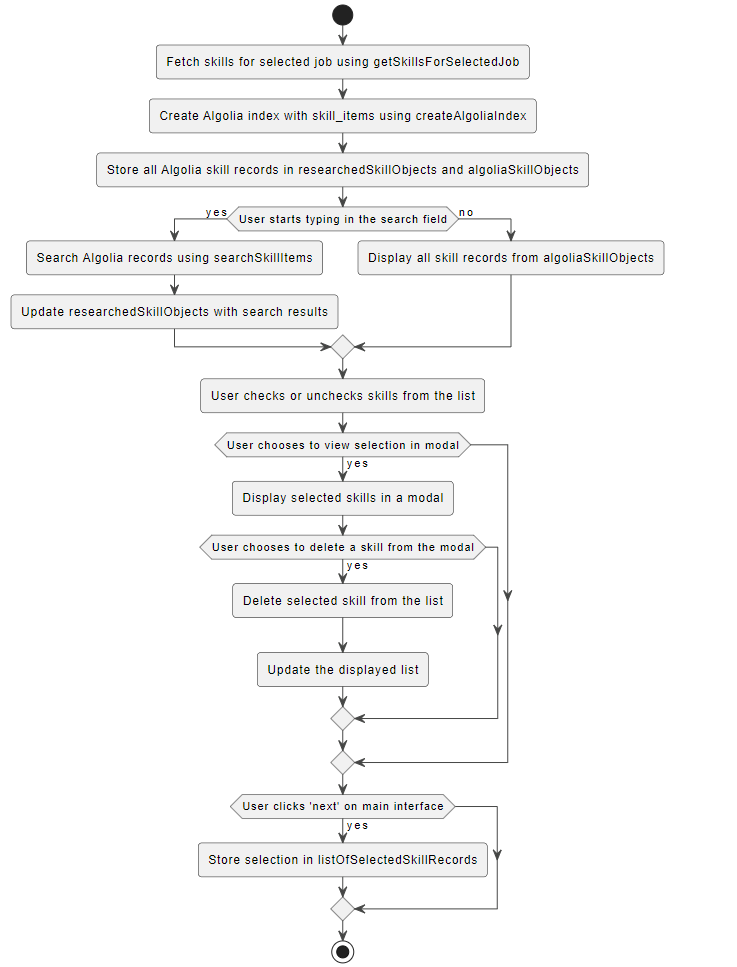
\includegraphics[width=\linewidth]{src/assets/images/sprint2UseCase2.png}}
    \caption{ Activity Diagram for the Filter and Select Skills for Chosen Job Category Use-Case }
    \label{fig:UseCase2Sprint2_Activity_Diagram}
\end{figure}

\subsection*{Description}
The second use case activity diagram thoroughly outlines the systematic process of searching for and selecting skills for a job, facilitating HR Managers to identify the specific skillset required for a given role.
The entire process is initiated by fetching the relevant skills for the selected job. This is achieved via the getSkillsForSelectedJob API call. The result of this API call is a list of skills related to the job, and these are promptly stored in the \verb|skill_items| index on Algolia. This storage not only keeps the data safe but also makes it readily searchable, leveraging Algolia's efficient search capabilities.
The system then proceeds to load all of the records from the Algolia index into two local variables, namely researchedSkillObjects and \verb|algoliaSkillObjects|. These hold the skill objects in a readily accessible manner for future steps.
If the HR Manager inputs a search query in the search field, the \verb|searchSkillItems| function is activated. This function uses the search query to search through the records in the Algolia index, providing a list of relevant skills. This list updates the \verb|researchedSkillObjects| variable, ensuring that the system is aware of the current search results. 
On the other hand, if the HR Manager doesn't input any query in the search field, all skill records from the algoliaSkillObjects variable are displayed, providing the full range of skills related to the selected job for the HR Manager to peruse. 
The HR Manager can then engage with the list of skills, checking off those that are relevant and unchecking those that are not. If the 'Show Selection' button is clicked, a modal is displayed that houses all the selected skills. In this modal, the HR Manager has the ability to review the selected skills and even delete any skill if necessary. The displayed list of skills is dynamically updated to reflect any such deletions.
The final step occurs when the HR Manager clicks on the 'Next' button. This action prompts the system to store the final selection of skills in the listOfSelectedSkillRecords variable. This ensures that the selection made by the HR Manager is saved and readily available for future steps or references within the application.


\subsubsection{Use Case 3: Fetch and Select Tasks for Chosen Skills} 
\begin{figure}[H]
    \centering
    \makebox[\textwidth]{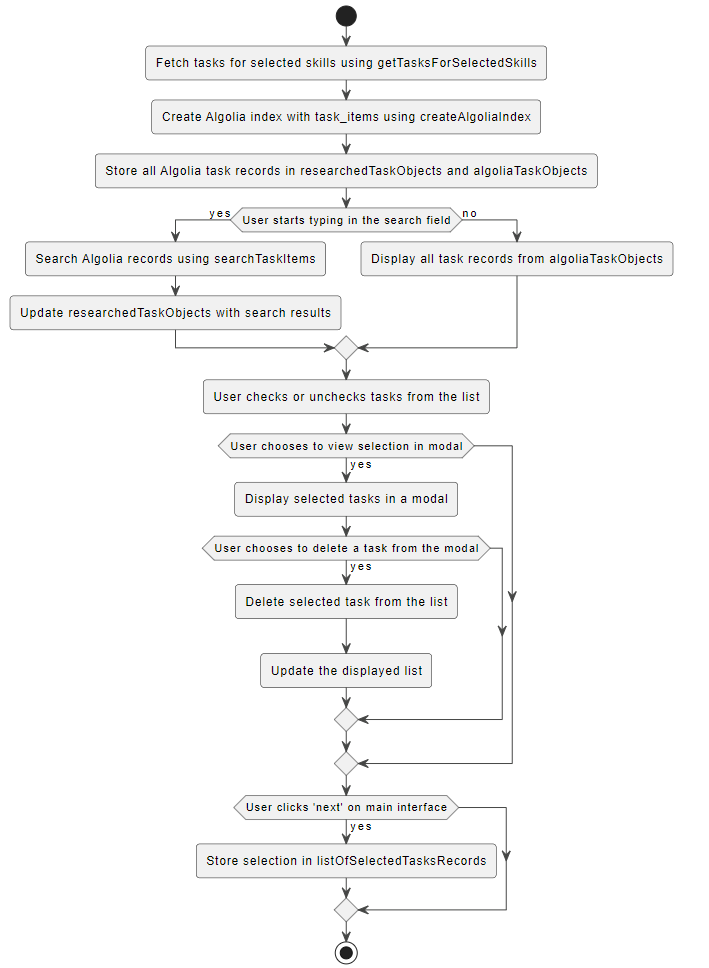
\includegraphics[width=\linewidth]{src/assets/images/sprint2UseCase3.png}}
    \caption{ Activity Diagram for the Fetch and Select Tasks for Chosen Skills Use-Case }
    \label{fig:UseCase3Sprint2_Activity_Diagram}
\end{figure}

\subsection*{Description}
The third use case activity diagram illustrates the procedure involved in seeking and selecting the tasks related to the skills pre-selected for a job. It is essentially a progression of steps tailored to offer the HR manager a systematic approach to defining the tasks of a job role.

This process is \verb|kick-started| by utilizing the getTasksForSelectedSkills API call, a function designed to pull out tasks associated with the previously selected skills for the given job. The fetched tasks are then integrated and stored in an Algolia index referred to as \verb|task_items|.

Following this, the Algolia index is processed to extract and store all records into two local variables, researchedTaskObjects and algoliaTaskObjects. This dual storage facilitates an effective search function. As the user inputs search terms into the search field, the function searchTaskItems sifts through the Algolia records and filters out corresponding results. These search results subsequently update the researchedTaskObjects variable. In the scenario where the user does not provide any input, all task records housed in algoliaTaskObjects are put on display.

Upon displaying the tasks, the user is given the liberty to check or uncheck tasks from the generated list. This action is aimed at selecting and deselecting tasks for the job. In order to review their selection, the user can opt to click on the 'show selection' button which prompts a modal to pop up displaying the selected tasks. If the user identifies a task that they wish to remove from the selection, they can simply delete it from this modal, which will cause the displayed task list to update automatically.

The final stage in this process occurs when the user selects the 'next' option. At this point, the system takes the selections made by the user and commits them into the listOfSelectedTasksRecords variable for future use in job description creation. Thus, with a series of methodical steps, the system enables the user to navigate through a vast array of tasks and select the ones most relevant to the job at hand.


\subsubsection{Use Case 4: Generate Job Description} 
\begin{figure}[H]
    \centering
    \makebox[1.2\textwidth]{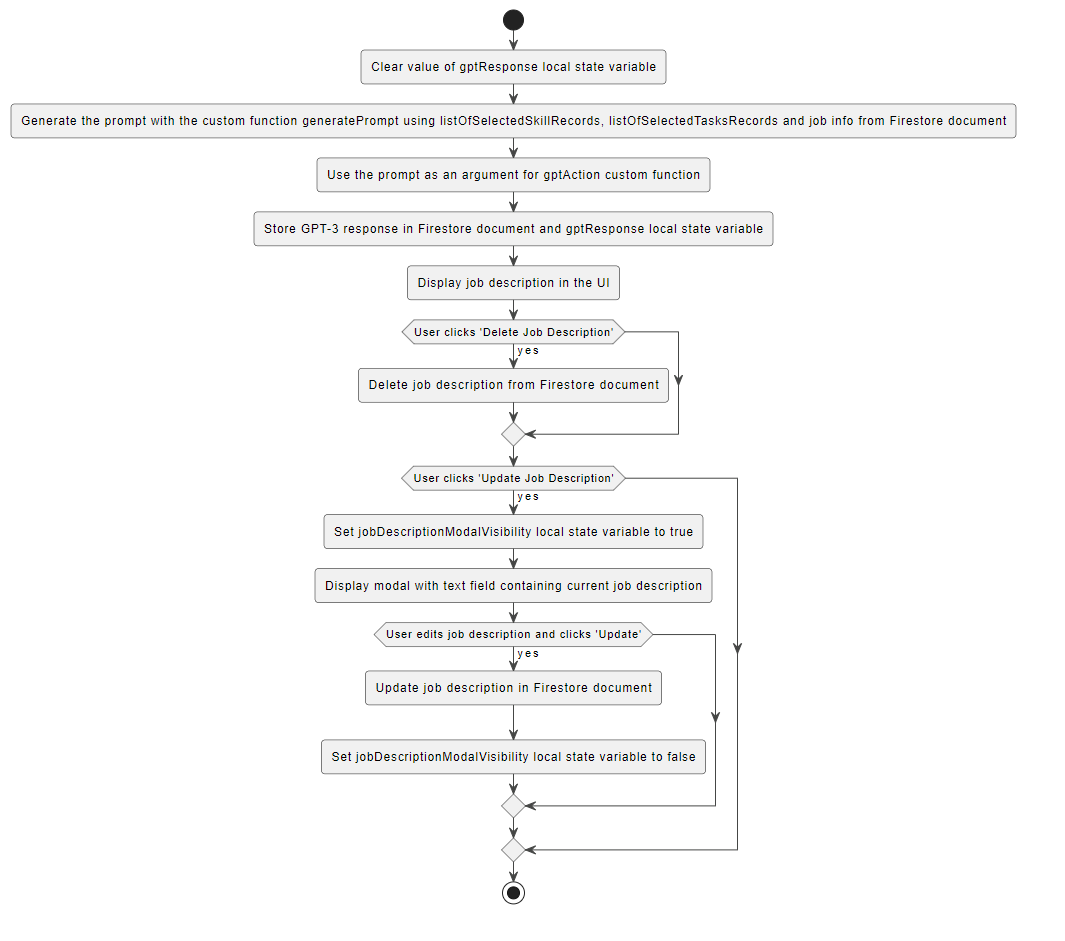
\includegraphics[width=1.4\linewidth]{src/assets/images/sprint2UseCase4.png}}
    \caption{ Activity Diagram for the Generate Job Description Use-Case }
    \label{fig:UseCase4Sprint2_Activity_Diagram}
\end{figure}

\newpage
\subsection*{Description}
The fourth use case's activity diagram meticulously charts the processes entailed in creating, displaying, altering, and discarding a job description.

At the onset, the local state variable gptResponse is reset to ensure no previous data influences the upcoming operation. Following this, a unique function titled generatePrompt is activated to generate a prompt. The inputs to this function comprise the listOfSelectedSkillRecords, listOfSelectedTasksRecords and specific job information extracted from the Firestore document. These details provide the context required to generate an appropriate job description.

Once the prompt is established, it serves as a parameter for the gptAction custom function. This function interacts with the GPT-3 model and receives a response. This response, essentially a draft job description, is stored in two locations - the Firestore document for data persistence and the gptResponse local state variable for real-time use. This job description is then presented to the user on the user interface.

The user is offered multiple avenues to modify this job description. The option to 'Delete Job Description' allows the user to completely remove the job description from the Firestore document, effectively discarding it. Conversely, the 'Update Job Description' button triggers a different process.

Clicking on 'Update Job Description' sets the jobDescriptionModalVisibility local state variable to true, invoking a modal populated with a text field that contains the current job description. The user can then edit this job description in real-time. On clicking 'Update', the revised job description replaces the original one in the Firestore document, ensuring the changes are saved for subsequent reference. This also leads to the closure of the modal by reverting jobDescriptionModalVisibility to false. This sequence of actions allows users to tailor the job description to their satisfaction.

\newpage
\subsection{Detailed Sequence Diagrams}
\subsubsection{Use Case 1: Select Job Category and Specialized Field} 

\begin{figure}[H]
    \centering
    \makebox[\textwidth]{\includegraphics[width=1.25\linewidth]{src/assets/images/SD-Select-Job.jpg}}
    \caption{ Sequence Diagram for the Select Job Category and Specialized Field Use-Case }
    \label{fig:UseCase1Sprint2_Sequence_Diagram}
\end{figure}

\newpage
\subsection*{Description}
The sequence diagram offers a comprehensive visual representation of the HR Manager's interactions to choose a job category and related fields within the HR management system.

Initiating the process, the system retrieves well-structured data from the 'jobList' table located within the Skill Dictionary of the Airtable database. This is achieved through the call of the custom function, fetchJobList(). The resulting data is stored in the Firestore database for future reference and manipulation, thus beginning the dynamic process of creating drop-down menus.

Following this, a sequence of cascading drop-down menus are populated based on the user's choices. This chain of actions is driven by a series of custom functions, each function depending on the outcome of its predecessor. The first dropdown corresponds to the 'Origin' field, which upon selection, informs the population of the subsequent dropdown for 'Personnel Category'.

This chain continues, with each selection impacting the next dropdown. The 'Personnel Type' dropdown is populated based on the 'Personnel Category' selected, and the chosen 'Personnel Type' informs the options of the 'Job Category' dropdown.

There's an additional conditional stage where, if the selected job category possesses any specialized fields, an extra dropdown for 'Specialized Fields' appears. The user's selection, if any, is recorded for future use. If the job category lacks specialized fields, this dropdown is bypassed entirely.

Each user interaction in the selection of a dropdown option triggers an update in the Firestore document pertaining to the job description. The Firestore document is thus continually updated with new data as the HR Manager progresses through the selection process.

Upon the conclusion of this interactive sequence, the HR Manager would have chosen all relevant fields in connection to the job category, thereby setting the groundwork for the next stages of the job creation process. The execution of this sequence diagram ensures the accurate and efficient collection of job-related information, streamlining the job creation process.


\newpage
\subsubsection{Use Case 2: Filter and Select Skills for Chosen Job Category} 

\begin{figure}[H]
    \centering
    \makebox[\textwidth]{\includegraphics[width=1.25\linewidth]{src/assets/images/SD-Select-Skills.jpg}}
    \caption{ Sequence Diagram for the Filter and Select Skills for Chosen Job Category Use-Case }
    \label{fig:UseCase2Sprint2_Sequence_Diagram}
\end{figure}

\newpage
\subsection*{Description}
The illustrated sequence diagram thoroughly visualizes the process by which the HR Manager selects skill items for a particular job within the HR management system.

Initiating this process, the system executes an HTTP request to the 'getSkillsForSelectedJob' API. This API, designed to fetch all skill elements related to a previously chosen job, gathers relevant data for use in subsequent steps. The resulting skills data set is then utilized for indexing in Algolia, a powerful and flexible search API. If an existing index for these skills already resides in Algolia, it is overwritten to maintain data integrity and freshness.

With the Algolia indexing operation complete, the system next carries out an action to retrieve all skill records indexed in Algolia. The fetchAllAlgoliaRecords function is employed for this task, yielding a complete set of skill records.

These records are then stored in two local state variables, researchedSkillObjects and algoliaSkillObjects, ensuring their availability for future reference and manipulation.

Once the data is stored, the HR Manager is equipped to search for specific skill items using the search field. The system provides assistance in this process through the searchSkillItems function, which sifts through the Algolia records to return search results. If the HR Manager does not provide input in the search field, all skill records stored in algoliaSkillObjects are displayed for review.

These skills are displayed in a ListView, a user-friendly interface that allows the HR Manager to visually navigate through the available skills. The manager can then check or uncheck desired skill items from this list. The selected skills are stored in another local state variable, listOfSelectedSkillRecords, capturing the HR Manager's choices for later use in the job description.

The sequence diagram concludes with the HR Manager's selection of skill items, which are stored for further processing in the job creation process. The successful execution of this sequence ensures that the most relevant skills are chosen for a particular job, contributing to the efficacy and accuracy of the job description.


\newpage
\subsubsection{Use Case 3: Fetch and Select Tasks for Chosen Skills} 

\begin{figure}[H]
    \centering
    \makebox[\textwidth]{\includegraphics[width=1.2\linewidth]{src/assets/images/SD-Select-Tasks.jpg}}
    \caption{ Sequence Diagram for the Fetch and Select Tasks for Chosen Skills Use-Case }
    \label{fig:UseCase3Sprint2_Sequence_Diagram}
\end{figure}

\newpage
\subsection*{Description}
The illustrated sequence diagram represents the intricate process by which the HR Manager selects task items related to the previously chosen skills within the HR management system. This flow is a logical continuation of the skill selection sequence that took place in the previous use case, therefore, it begins by referencing that sequence.

Commencing this process, the system executes an HTTP request to the 'getTasksForSelectedSkills' API. This API, designed to fetch all tasks correlated with the selected skills, extracts relevant data and passes the selected skills as arguments to ensure a relevant response.

Upon receiving the tasks from the API, a custom action named createAlgoliaIndexForTasks is invoked. This action's main function is to create or overwrite an index in the Algolia database, which is a flexible and powerful search API. The index is named \verb|task_items| and serves as the storage location for task data to facilitate rapid retrieval and search functionality.

With the Algolia indexing operation complete, the system next initiates another custom action named returnAllAlgoliaTaskRecords. This function is responsible for retrieving all the records indexed in Algolia and makes the task data readily available for the subsequent operations.

The retrieved records are then stored in two local state variables: researchedTaskObjects and algoliaTaskObjects. These variables not only preserve the data for future reference and manipulation but also enable the display of tasks in the ListView interface.

Now that the data is available, the HR Manager can conduct a search for specific tasks or select tasks directly from the displayed list. The system assists the user by enabling the searchTaskItems function, which scours the Algolia records to yield search results based on the user's input.

Finally, the selected tasks are recorded in the listOfSelectedTasksRecords local state variable. This variable serves as a storage bin for the HR Manager's selections, allowing the choices to be utilized in the subsequent use case - the generation of a job description.

The sequence diagram concludes with the HR Manager's selection of task items, setting the stage for the next steps in the job creation process. The successful execution of this sequence ensures that the most pertinent tasks are chosen based on the previously selected skills, further enhancing the accuracy of the job description.

\newpage
\subsubsection{Use Case 4: Generate Job Description} 

\begin{figure}[H]
    \centering
    \makebox[\textwidth]{\includegraphics[width=1.2\linewidth]{src/assets/images/SD-Generate-Job-Description.jpg}}
    \caption{ Sequence Diagram for the Generate Job Description Use-Case }
    \label{fig:UseCase4Sprint2_Sequence_Diagram}
\end{figure}

\newpage
\subsection*{Description}
This sequence diagram illustrates the comprehensive process of generating a job description, a crucial task for the HR Manager in the HR management system.

The process begins with an initial housekeeping step, clearing the existing value, if any, from the local state variable gptResponse. This action ensures that there are no remnants from any previous job description generation processes that might interfere with the current task.

Next, the system initiates the gptAction custom action. This complex action is responsible for creating a well-crafted prompt that will be used as input for the GPT-3.5-turbo model. The creation of this prompt involves an intricate concatenation of various data elements, including the selected skills, tasks, job comments, and the job category, each obtained from their respective local state variables or Firestore documents. The carefully constructed prompt encapsulates the essential attributes required for a comprehensive job description.

Upon successful generation of the prompt, the system makes an API call to the GPT-3.5-turbo model, passing the prompt as an argument. Leveraging the advanced AI of GPT-3.5-turbo, the system generates a detailed, nuanced job description based on the information contained in the prompt.

The job description, returned by the GPT-3.5-turbo model, is then stored in two places: a Firestore document and the gptResponse local state variable. Storing the description in Firestore facilitates persistent data storage, while placing it in gptResponse allows the system to display the job description to the HR Manager on the user interface.

Upon viewing the generated job description, the HR Manager is offered two choices: delete or update the job description. In the event the HR Manager elects to delete the job description, a simple action is performed to remove it from the Firestore document. However, if the HR Manager chooses to update the description, a more complex series of steps ensue.

Firstly, the jobDescriptionModalVisibility local state variable is set to true, causing a modal containing the current job description to appear on the interface. Within this modal, the HR Manager can edit the description as needed. Once satisfied with the revisions, the HR Manager clicks 'Update', causing the updated job description to replace the old one in the Firestore document. Finally, the modal is closed by setting jobDescriptionModalVisibility back to false, signaling the end of the job description generation process.


\section{Implementation}
In this sprint, the main goal was to allow HR Managers to select a job category and the associated specialized field. This involved creating functionalities for users to interact with dynamic dropdowns and fetch relevant data from the Airtable database.

\subsection{Dynamic Dropdown Feature} 
The first step was to design and implement a dynamic dropdown feature for job category selection. This involved creating a user interface with multiple dropdown menus where HR Managers could select an origin, a personnel category, a personnel type, a job category, and if available, a specialized field.

The backend functionality was then developed to fetch the relevant data for each dropdown based on the user's previous selections. This involved setting up the connection with the Airtable database and writing the necessary server-side code to handle the data retrieval process.


\begin{figure}[H]
    \centering
    \makebox[\textwidth]{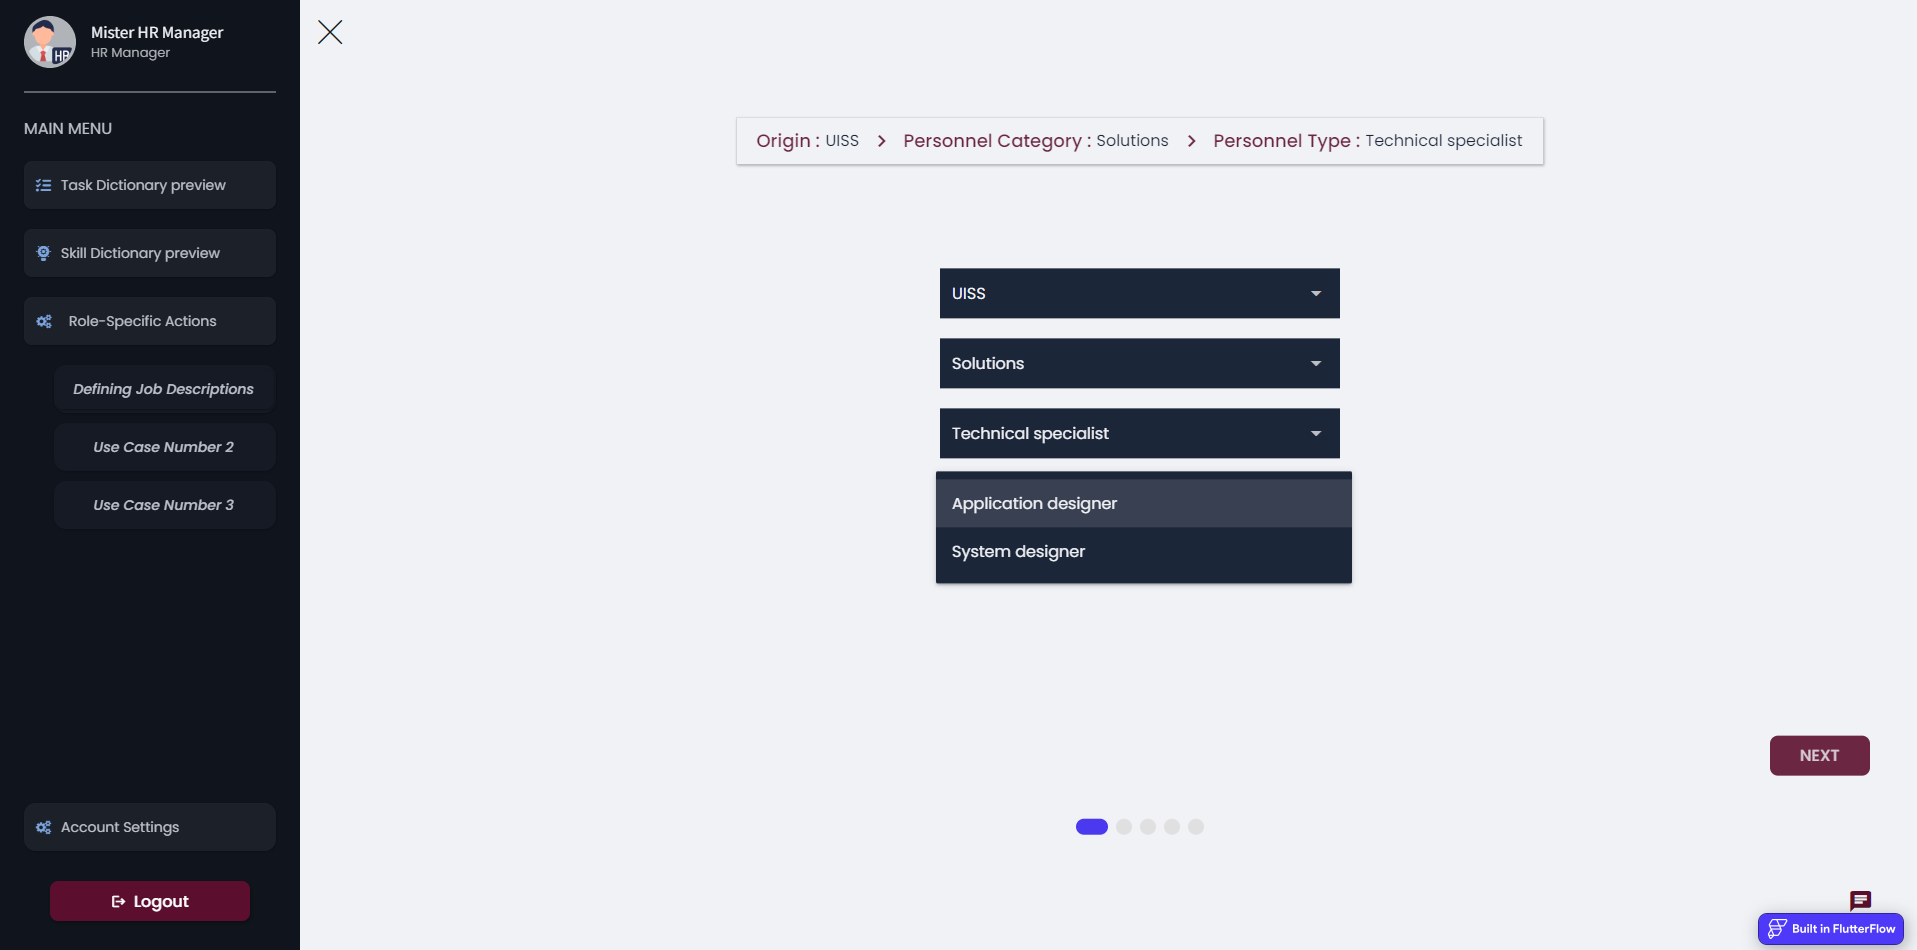
\includegraphics[width=1.2\linewidth]{src/assets/images/sprint2_DropdDowns.PNG}}
    \caption{ Dynamic Dropdown Feature overview page}
    \label{fig:Dynamic-Dropdown-Feature-overview-page}
\end{figure}


\newpage
\subsection{Skill Filtering and Selection} 
The next step was to design and implement a feature that fetches skills related to the selected job category (and specialized field if selected) from the Airtable database. This involved creating a user interface where HR Managers could filter and search through the skills using Algolia search engine capabilities.

The backend functionality was then developed to fetch the relevant skills from the Airtable database and handle the search and filter requests from the Algolia search engine.

\begin{figure}[H]
    \centering
    \makebox[\textwidth]{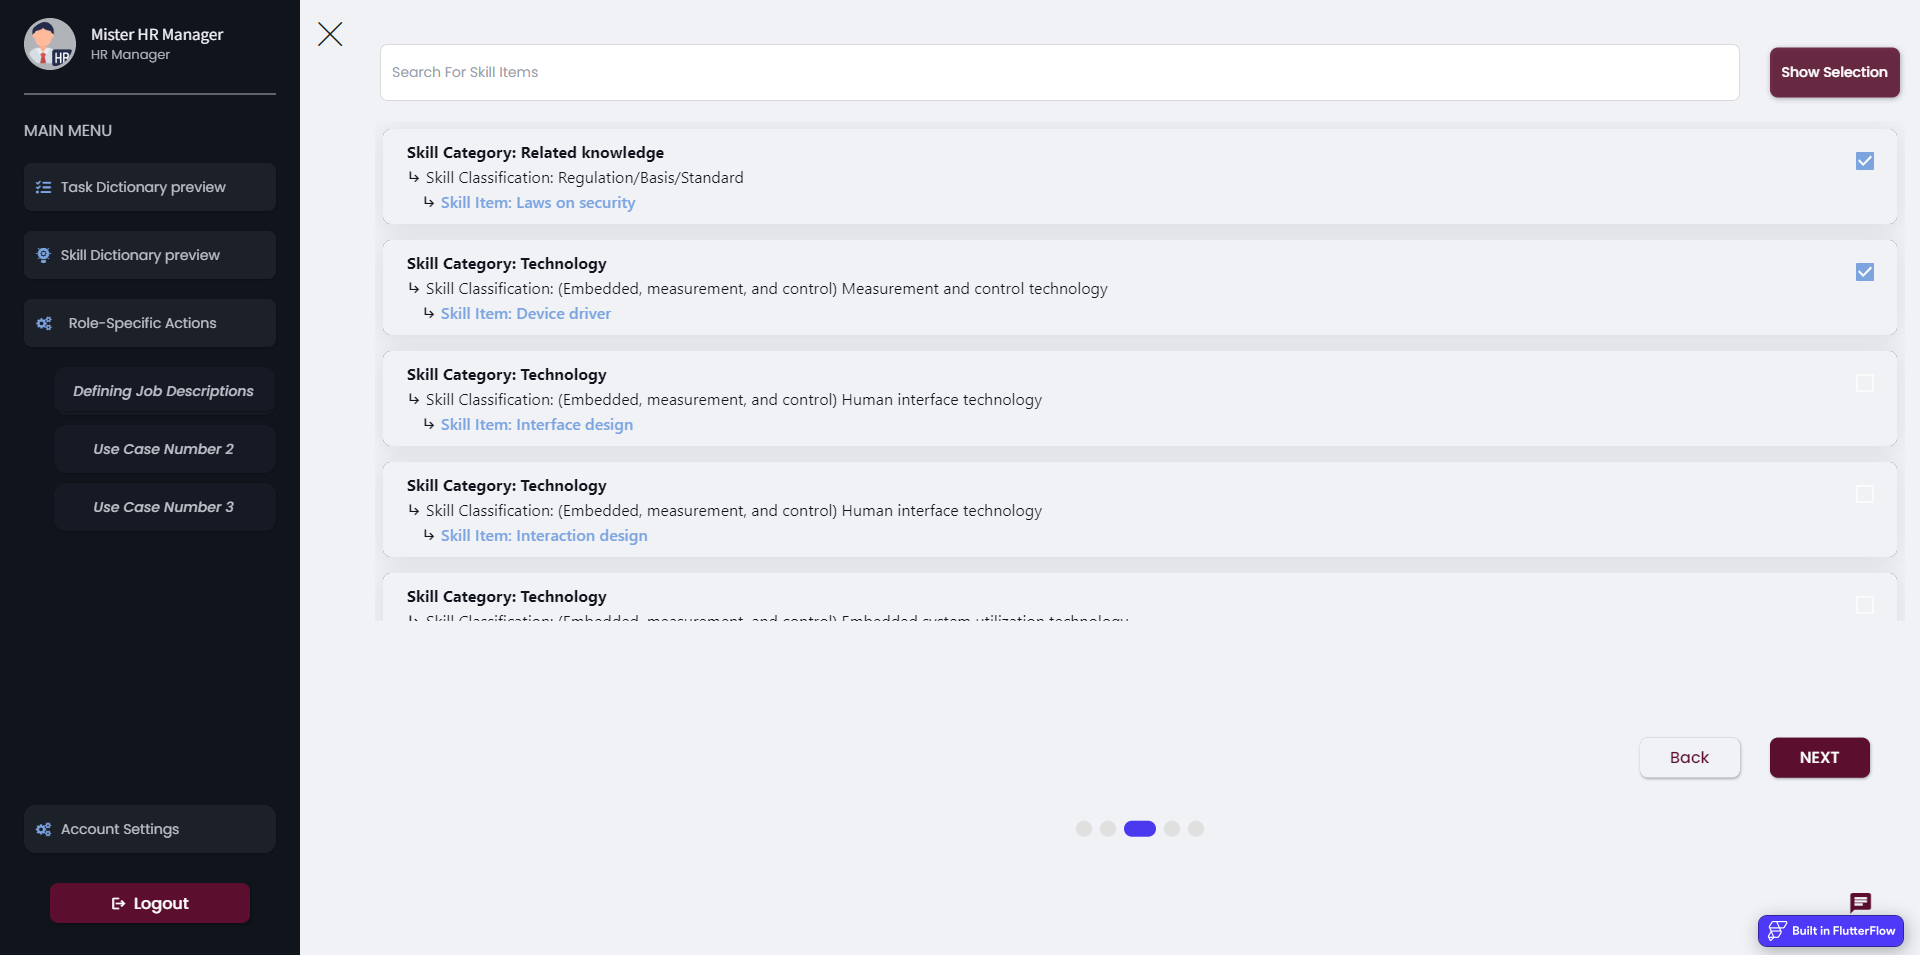
\includegraphics[width=1.2\linewidth]{src/assets/images/sprint2_SkillSelection.PNG}}
    \caption{ Skill Filtering and Selection overview page}
    \label{fig:Skill-Filtering-and-Selection-overview-page}
\end{figure}


\newpage
\subsection{Task Filtering and Selection} 
The third step was to design and implement a feature that fetches tasks related to the selected skills from the Airtable database. This involved creating a user interface where HR Managers could filter and search through the tasks using Algolia search engine capabilities.

The backend functionality was then developed to fetch the relevant tasks from the Airtable database and handle the search and filter requests from the Algolia search engine.

\begin{figure}[H]
    \centering
    \makebox[\textwidth]{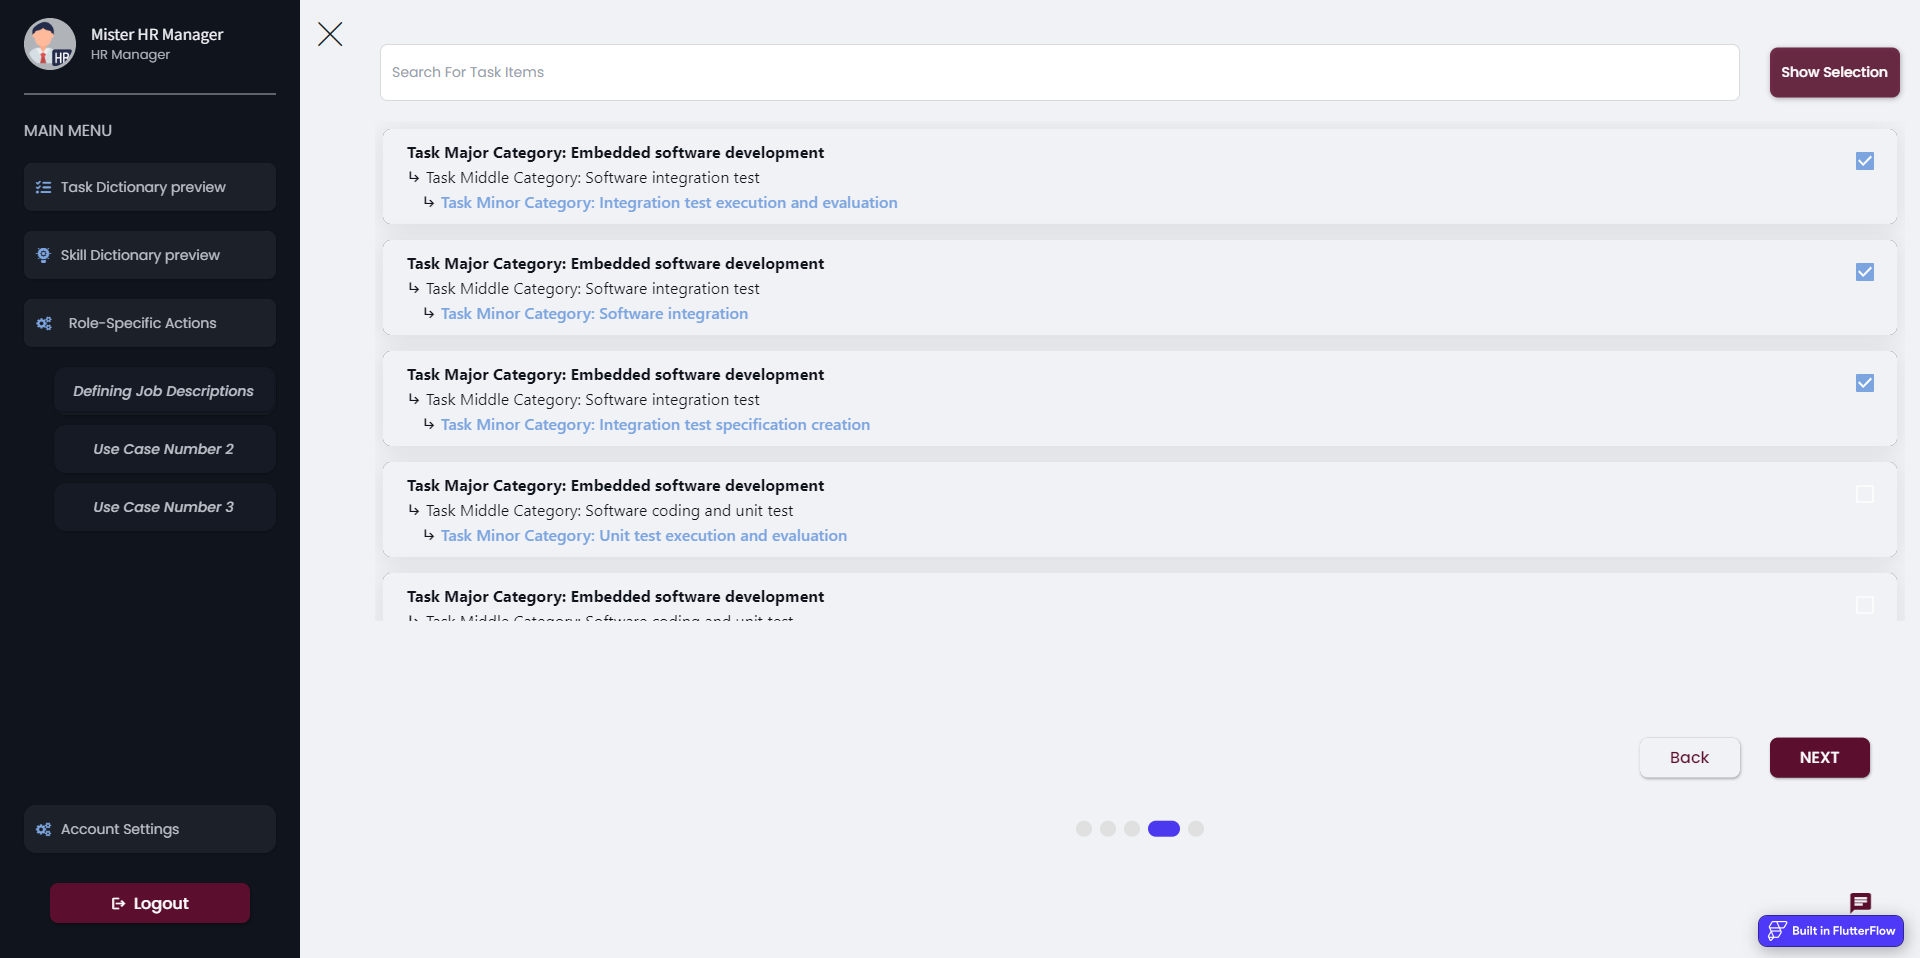
\includegraphics[width=1.2\linewidth]{src/assets/images/sprint2_TaskSelection.PNG}}
    \caption{ Task Filtering and Selection overview page}
    \label{fig:Task-Filtering-and-Selection-overview-page}
\end{figure}

\newpage
\subsection{Job Description Generation} 
The final step was to implement a feature that generates a job description using the GPT-3 API based on the selected skills and tasks. This involved writing server-side code to call the GPT-3 API with the selected skills and tasks as input and receive the generated job description as output.

The generated job description was then displayed to the HR Manager, who could download, print, modify, regenerate, or delete it. Any modification or new generation of job description was saved in the Firestore database.


\begin{figure}[H]
    \centering
    \makebox[\textwidth]{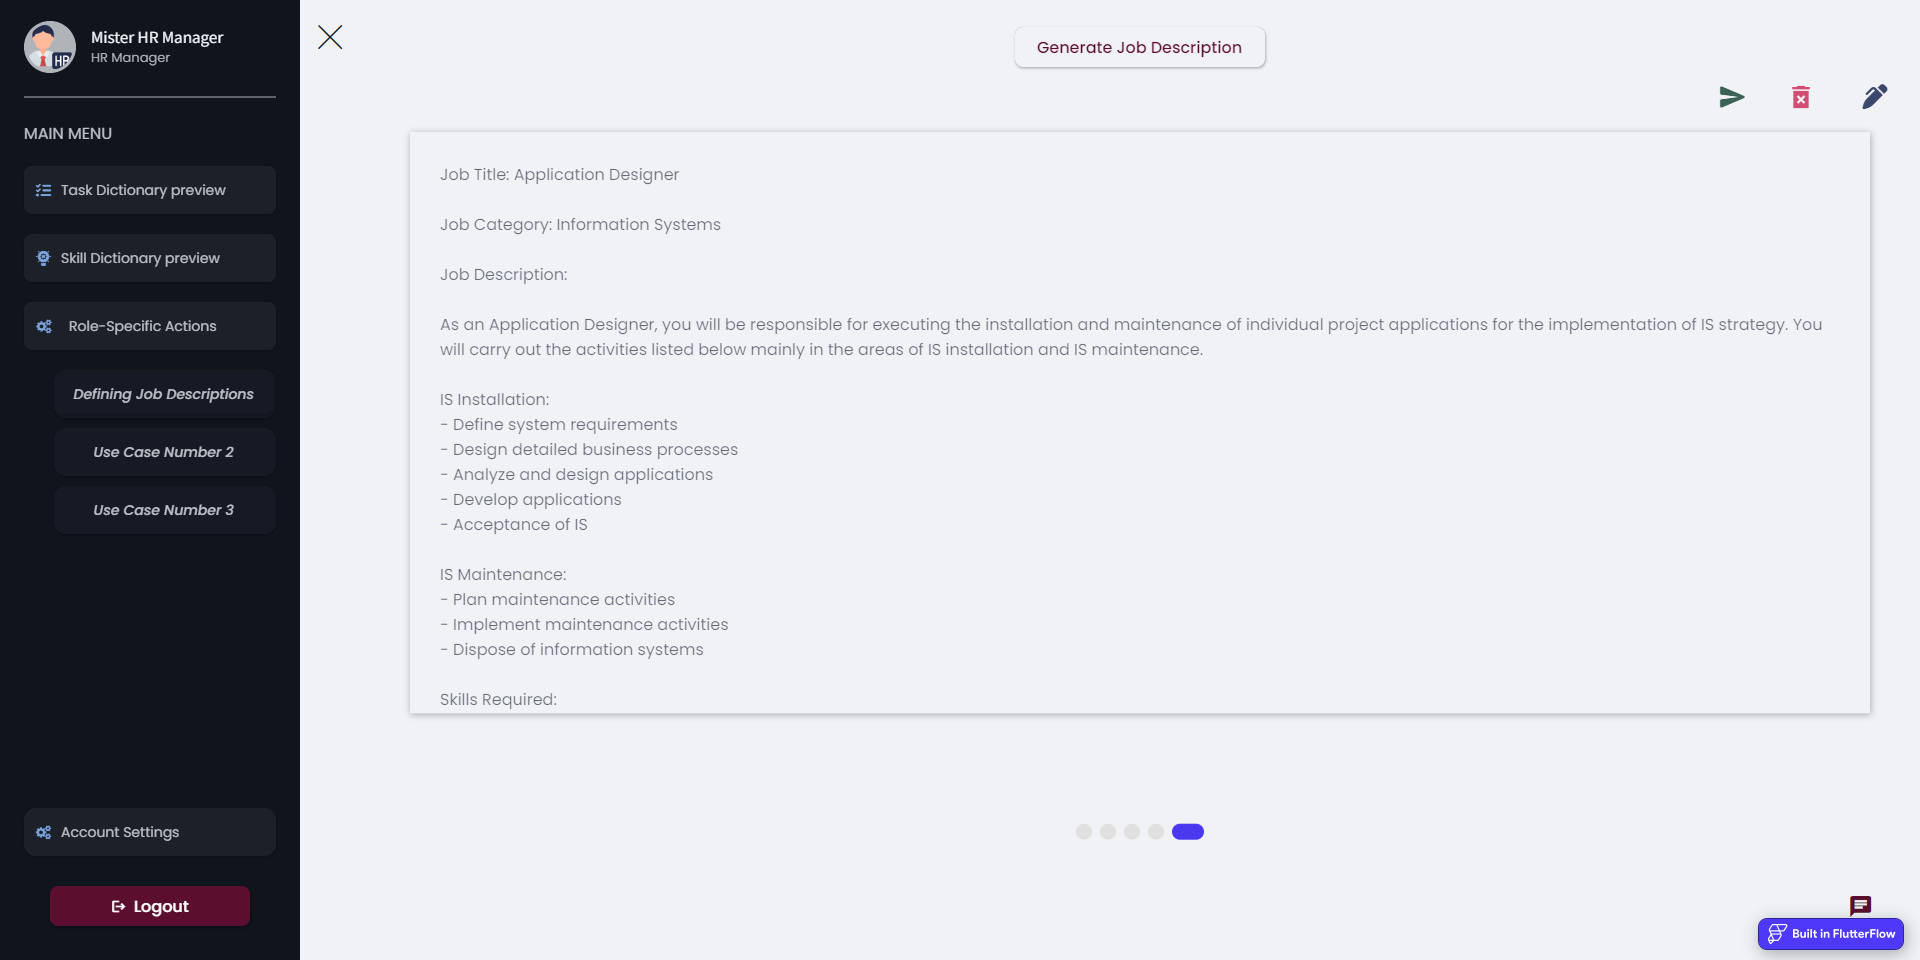
\includegraphics[width=1.2\linewidth]{src/assets/images/sprint2_GenerateJobDescription.PNG}}
    \caption{ Job Description Generation overview page}
    \label{fig:Job-Description-Generation-overview-page}
\end{figure}


\subsection{Integration and Testing}
After developing these features, they were integrated into the system, ensuring smooth interaction with other features and data. Comprehensive testing was carried out to ensure functionality and to rectify any identified issues.

This marks the completion of the second sprint, effectively enabling HR Managers to define roles and responsibilities through job categories, specialized fields, skills, tasks, and comprehensive job description generation.


